% Options for packages loaded elsewhere
\PassOptionsToPackage{unicode}{hyperref}
\PassOptionsToPackage{hyphens}{url}
%
\documentclass[
]{article}
\usepackage{amsmath,amssymb}
\usepackage{lmodern}
\usepackage{iftex}
\ifPDFTeX
  \usepackage[T1]{fontenc}
  \usepackage[utf8]{inputenc}
  \usepackage{textcomp} % provide euro and other symbols
\else % if luatex or xetex
  \usepackage{unicode-math}
  \defaultfontfeatures{Scale=MatchLowercase}
  \defaultfontfeatures[\rmfamily]{Ligatures=TeX,Scale=1}
\fi
% Use upquote if available, for straight quotes in verbatim environments
\IfFileExists{upquote.sty}{\usepackage{upquote}}{}
\IfFileExists{microtype.sty}{% use microtype if available
  \usepackage[]{microtype}
  \UseMicrotypeSet[protrusion]{basicmath} % disable protrusion for tt fonts
}{}
\makeatletter
\@ifundefined{KOMAClassName}{% if non-KOMA class
  \IfFileExists{parskip.sty}{%
    \usepackage{parskip}
  }{% else
    \setlength{\parindent}{0pt}
    \setlength{\parskip}{6pt plus 2pt minus 1pt}}
}{% if KOMA class
  \KOMAoptions{parskip=half}}
\makeatother
\usepackage{xcolor}
\usepackage[margin=1in]{geometry}
\usepackage{longtable,booktabs,array}
\usepackage{calc} % for calculating minipage widths
% Correct order of tables after \paragraph or \subparagraph
\usepackage{etoolbox}
\makeatletter
\patchcmd\longtable{\par}{\if@noskipsec\mbox{}\fi\par}{}{}
\makeatother
% Allow footnotes in longtable head/foot
\IfFileExists{footnotehyper.sty}{\usepackage{footnotehyper}}{\usepackage{footnote}}
\makesavenoteenv{longtable}
\usepackage{graphicx}
\makeatletter
\def\maxwidth{\ifdim\Gin@nat@width>\linewidth\linewidth\else\Gin@nat@width\fi}
\def\maxheight{\ifdim\Gin@nat@height>\textheight\textheight\else\Gin@nat@height\fi}
\makeatother
% Scale images if necessary, so that they will not overflow the page
% margins by default, and it is still possible to overwrite the defaults
% using explicit options in \includegraphics[width, height, ...]{}
\setkeys{Gin}{width=\maxwidth,height=\maxheight,keepaspectratio}
% Set default figure placement to htbp
\makeatletter
\def\fps@figure{htbp}
\makeatother
\setlength{\emergencystretch}{3em} % prevent overfull lines
\providecommand{\tightlist}{%
  \setlength{\itemsep}{0pt}\setlength{\parskip}{0pt}}
\setcounter{secnumdepth}{5}
\ifLuaTeX
  \usepackage{selnolig}  % disable illegal ligatures
\fi
\IfFileExists{bookmark.sty}{\usepackage{bookmark}}{\usepackage{hyperref}}
\IfFileExists{xurl.sty}{\usepackage{xurl}}{} % add URL line breaks if available
\urlstyle{same} % disable monospaced font for URLs
\hypersetup{
  pdftitle={Efficient Frontier},
  pdfauthor={Ana Karapetrovic-Suput},
  hidelinks,
  pdfcreator={LaTeX via pandoc}}

\title{Efficient Frontier}
\author{Ana Karapetrovic-Suput}
\date{21. September 2022}

\begin{document}
\maketitle

\newpage 
\tableofcontents 
\listoftables
\newpage

\hypertarget{efficient-frontier}{%
\section{Efficient Frontier}\label{efficient-frontier}}

If you are thinking about investing in stocks, you will come across the
term ``efficient frontier''. The efficient frontier is the set of
optimal portfolios that offer the highest expected return for a defined
level of risk or the lowest risk for a given level of expected return.
If you choose the portfolio with the lower risk or the higher expected
return, depends on how risk-averse or risk-taking you are as an
investor. In the example below I chose 5 stocks for my portfolio. The
following stocks were used at the beginning: AMZN, AAPL, NFLX, XOM, T.
You can replace the stocks with any other you like. For more information
visit \url{https://finance.yahoo.com/}. There you can also find the
symbols of different stocks.

In the picture below you can see the ``Minimum Variance Portfolio'' as
well as the ``Tangency Portfolio''. The ``Minimum Variance Portfolio''
gives you a relative low return, but you have a low risk. If you choose
the ``Tangency Portfolio'' you can earn more money, but its riskier.

\begin{center}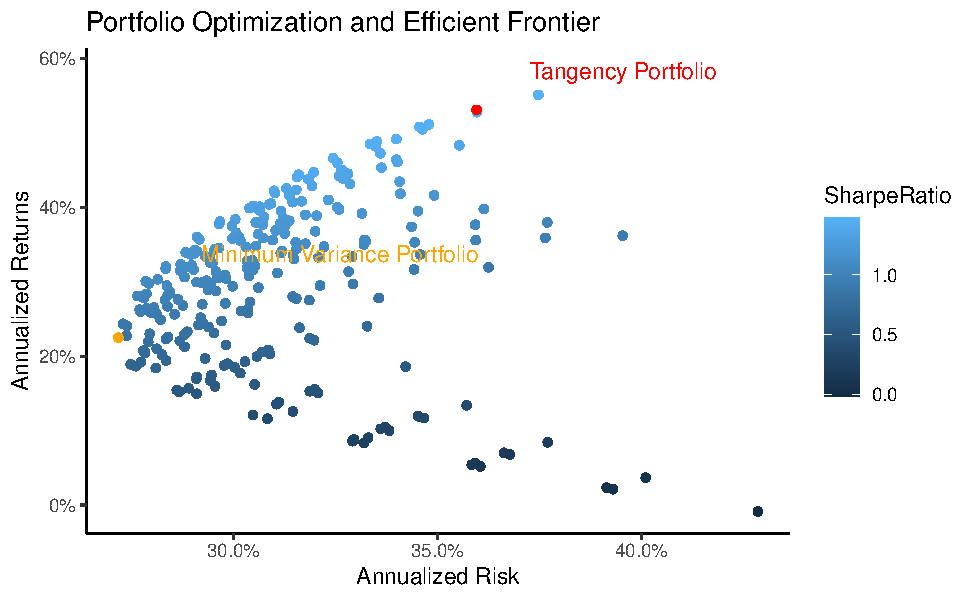
\includegraphics{EfficientFrontier_files/figure-latex/plot efficient frontier-1} \end{center}

\newpage

\hypertarget{minimum-variance-portfolio}{%
\section{Minimum Variance Portfolio}\label{minimum-variance-portfolio}}

The details for the portfolio with the lowest risk are shown below. It
is the portfolio with the lowest variance.

\begin{longtable}[]{@{}lllllll@{}}
\caption{Minimum Variance Portfolio - Weights, Return, Risk and Sharpe
Ratio}\tabularnewline
\toprule()
AAPL & AMZN & NFLX & T & Return & Risk & SharpeRatio \\
\midrule()
\endfirsthead
\toprule()
AAPL & AMZN & NFLX & T & Return & Risk & SharpeRatio \\
\midrule()
\endhead
10\% & 20\% & 10\% & 60\% & 16,5\% & 18,9\% & 0,869 \\
\bottomrule()
\end{longtable}

\begin{center}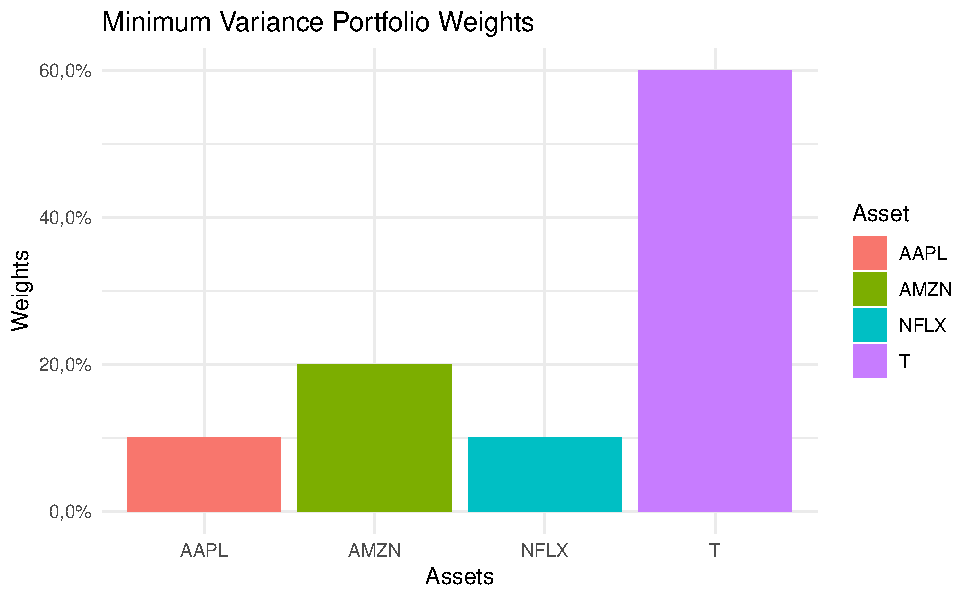
\includegraphics{EfficientFrontier_files/figure-latex/plot Minimum Variance Portfolio-1} \end{center}

\newpage

\hypertarget{tangency-portfolio}{%
\section{Tangency Portfolio}\label{tangency-portfolio}}

The details for the portfolio with the highest sharpe ratio are shown
below. The sharpe ratio seeks to characterize how well the return of an
asset compensates the investor for the risk taken. When comparing two
assets, the one with a higher sharpe ratio provides better return for
the same risk, which is usually attractive to investors.

\begin{longtable}[]{@{}lllllll@{}}
\caption{Tangency Portfolio - Weights, Return, Risk and Sharpe
Ratio}\tabularnewline
\toprule()
AAPL & AMZN & NFLX & T & Return & Risk & SharpeRatio \\
\midrule()
\endfirsthead
\toprule()
AAPL & AMZN & NFLX & T & Return & Risk & SharpeRatio \\
\midrule()
\endhead
30\% & 50\% & 20\% & 0\% & 38,7\% & 26,5\% & 1,463 \\
\bottomrule()
\end{longtable}

\begin{center}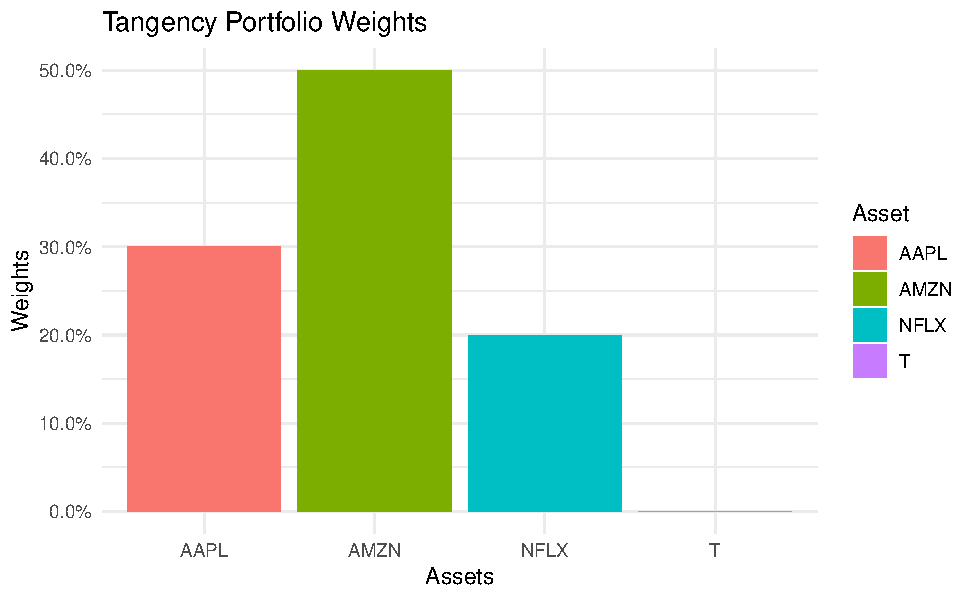
\includegraphics{EfficientFrontier_files/figure-latex/plot Tangency Portfolio-1} \end{center}

\end{document}
